\documentclass[a4paper,11pt, french]{article}
\usepackage[english]{babel}
\usepackage[utf8]{inputenc}
\usepackage{multicol}
\usepackage{graphicx}
\usepackage{float} 
\usepackage{fullpage}
\usepackage{algorithm}
\usepackage{algorithmic}
\usepackage{titlesec}
\usepackage{caption}
\usepackage{subcaption}
%\usepackage{titlesec}
\usepackage{tikz}
\usepackage[left=2.5cm, right=2.5cm, top=3cm, bottom=3cm]{geometry}
\usepackage{graphicx}
\usepackage{caption}
\usepackage{subcaption}
\usetikzlibrary{arrows}
\usepackage{bm}
\usepackage{latexsym}
\usepackage{amsmath}
\bibliographystyle{plain}

\usepackage{hyperref}
\renewcommand{\thesubsection}{Stage \Alph{subsection}}
\renewcommand{\thesubsubsection}{Q\Roman{section}.\Alph{subsection}.\arabic{subsubsection}}
\renewcommand{\thesection}{Part \arabic{section}}


\begin{document}

\title{Crowd Counting with CNN}
\author{Judith Abécassis, Timothée Lacroix, Arthur Mensch} 
\date{\today}
\maketitle
\section*{Introduction}
We compared two methods for estimating crowd count in images. We tried substituting SIFT with CNN in the method described in \cite{basepaper}, as well as in the multisource method proposed in \cite{multisource}, in the hope that this would lead to better results.

\section*{Two methods}
\subsection*{MESA distance regression}
The rationale is to use a specifically designed loss function \cite{basepaper}, the MESA distance,  in an optimisation problem to minimize the mismatches between the ground truth and the estimated density function. The optimal weight vector learnt on the training data can produce a density estimate for a new unseen image.

To plug the CNN features into this pipeline, we have used a pre-trained neural network \cite{overfeat}, modified to produce one feature per pixel (dense CNN). This was achieved by removing all pooling layers and set all stride parameters to 1 in the convolution layers. Several combinations of convolution (from 2 to 6) were tested.

\subsection*{Multiple Source Aggregation with $\epsilon$-SVR}
In this method, three sorts of features are generated: head detection (HOG), Fourier and sparse SIFT. Three distinct SVMs are then trained for each type of feature, and then a fourth SVM is trained to combine all of them. To plug CNN features in this framework, we have tried to replace sparse SIFT by CNNs computed as was detailed in the previous section.

\section*{Results}
\subsection*{Cells}
For the cells dataset \cite{basepaper}, we only evaluated the method from \cite{basepaper}, and its counterpart with CNNs. We followed the exact protocol from their paper to have comparable results. In each case, $N$ images (with $1 \leq N \leq 32$) are selected for the training dataset, another $N$ constitute a set to cross validate the regularization parameter of the method, and 100 images constitute the test set. For each value of $N$, 5 independent draws of test/train/validation sets were made.


\begin{table}[H]
\centering
    \begin{tabular}{|c|c|c|c|c|c|c|}
    \hline
    Validation & $N=1$ & $N=2$ & $N=4$ & $N=8$ & $N=16$ & $N=32$ \\ \hline
    counting & $12.7 \pm 7.3$ & $7.8 \pm 3.7$ & $5.0 \pm 0.5$ & $4.6 \pm 0.6$ & $4.2 \pm 0.4$ & $3.6 \pm 0.2$ \\ \hline
    MESA & $9.5 \pm 6.1$ & $6.3 \pm 1.2$ & $4.9 \pm 0.6$ & $4.9 \pm 0.7$ & $3.8 \pm 0.2$ & $3.5 \pm 0.2$ \\ \hline
    \end{tabular}
  \label{lempitskcell}
  \caption{Results presented in the article \cite{basepaper}}
\end{table}

\vspace{-0.5cm}
\begin{table}[H]
\centering
  \begin{tabular}{|c|c|c|c|c|c|c|}
  \hline
  Validation & $N=1$ & $N=2$ & $N=4$ & $N=8$ & $N=16$ & $N=32$ \\ \hline
  counting & $28.6 \pm 11.6$ & $16.4 \pm 4.4$ & $8.5 \pm 1.1$ & $7.2 \pm 0.9$ & $6.5 \pm 0.5$ & $5.5 \pm 0.5$ \\ \hline
  MESA & $26.1 \pm 5.2$ & $13.5 \pm 2.7$ & $8.9 \pm 1.4$ & $6.7 \pm 0.5$ & $6.9 \pm 0.3$ & $5.5 \pm 0.3$ \\ \hline
  \end{tabular}
  \label{lempitskcellour}
  \caption{Results we reproduced using the author's code}
\end{table}

\vspace{-0.5cm}
\begin{table}[H]
  \centering
  \begin{tabular}{|c|c|c|c|c|c|}
  \hline
  & NET 1 & NET 2 & NET 3 & NET 4 & NET 5 \\
  nFeatures & $N=16$ & $N=16$ & $N=16$ & $N=16$ & $N=16$  \\ \hline
  256 & $3.7 \pm 0.3$ & $3.8 \pm 0.4$ & $3.7 \pm 0.1$ & $3.9 \pm 0.2$ & $3.8 \pm 0.4$ \\ \hline
  512 & $3.4 \pm 0.2$ & $3.5 \pm 0.3$ & $3.7 \pm 0.2$ & $3.5 \pm 0.3$ & $3.6 \pm 0.2$ \\ \hline
  \end{tabular}
  \label{cnncell}
  \caption{Our results for $N=16$ ,different vocabulary size and different output CNN layer. }
\end{table}

There doesn't seem to be much improvement when considering deeper layers in the net. This was to be expected, considering how far the cells dataset is from the original training images of the CNN (imagenet).
Our results using CNN features are much better than those we reproduced using SIFTs, and a bit better than those reported by authors \cite{basepaper}.

\subsection*{Crowd}

We applied the algorithms from Lempitsky et al. \cite{basepaper} , Idrees et al. \cite{multisource} and our CNN version of Lempitsky to the dataset of crowds. For this dataset, the output layer that gave the best results was the $6th$, since images are closer to those encountered in the ImageNet training set. Our results are presented, split by total image count in figure~\ref{fig_compare}, as was done in \cite{multisource}, and averaged over all images in table~\ref{adcrowd}

\begin{figure}[H]
  \centering
  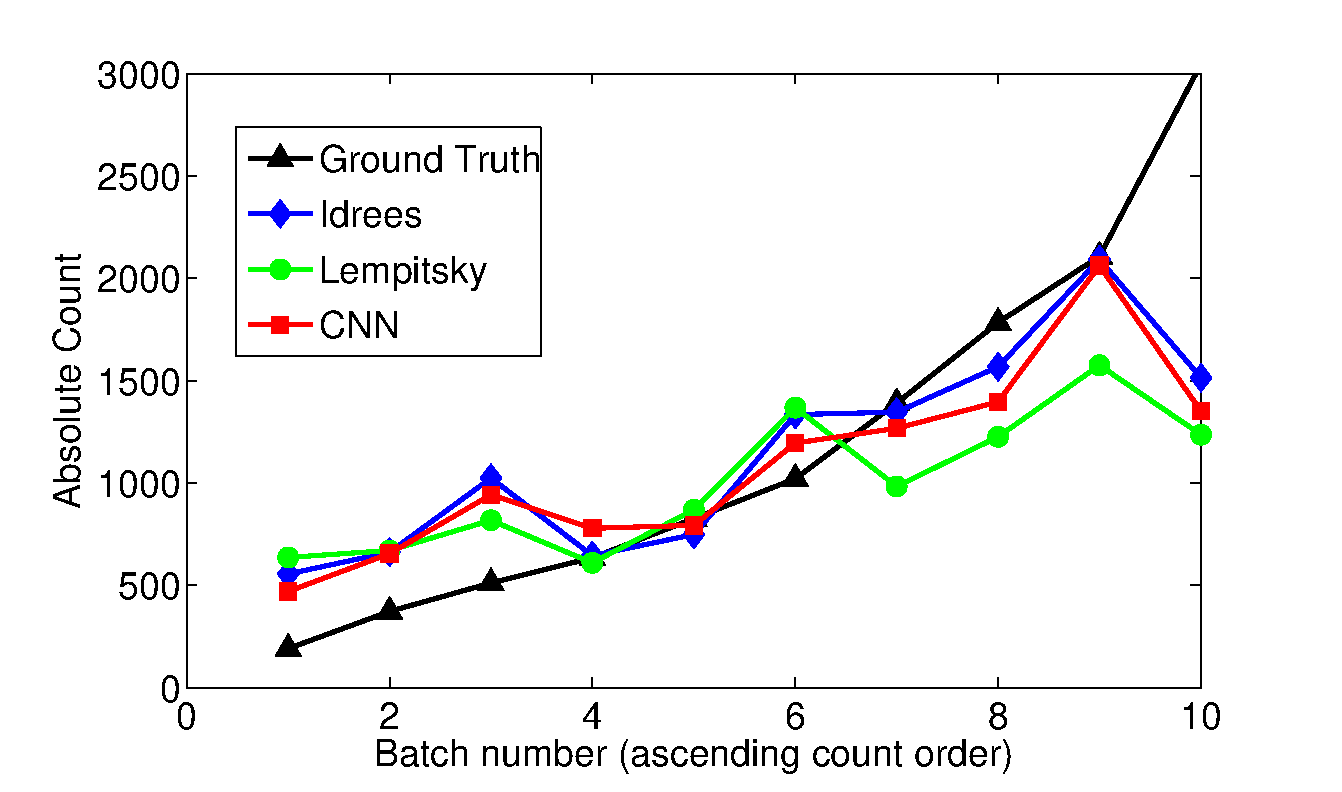
\includegraphics[width=0.9\textwidth]{figures/good_compare.eps}
  \caption{Comparison of Average Absolute Error for groups of $5$ images with same total count}
  \label{fig_compare}
\end{figure}

\begin{table}[H]
 \centering
  \begin{tabular}{|c|c|}
    \hline
    Lempitsky & $523 \pm 603$  \\ \hline
    Idrees & $466 \pm 481$  \\ \hline
    CNN & $464 \pm 516$  \\ \hline
  \end{tabular}
  
  \caption{Average Absolute Error on the crowd dataset for three methods}
  \label{adcrowd}
\end{table}


\subsection*{Short word on MRF}
We implemented our own multi-scale MRF as described in \cite{multisource, mrf}. But the corrections it led to were too small considering the amplitude of the errors, and the results of our algorithms were already quite continuous. Applying the MRF didn't lead to any noticeable improvements in the absolute count.
\begin{figure}[h!]
        \centering
        \begin{subfigure}[b]{0.3\textwidth}
	  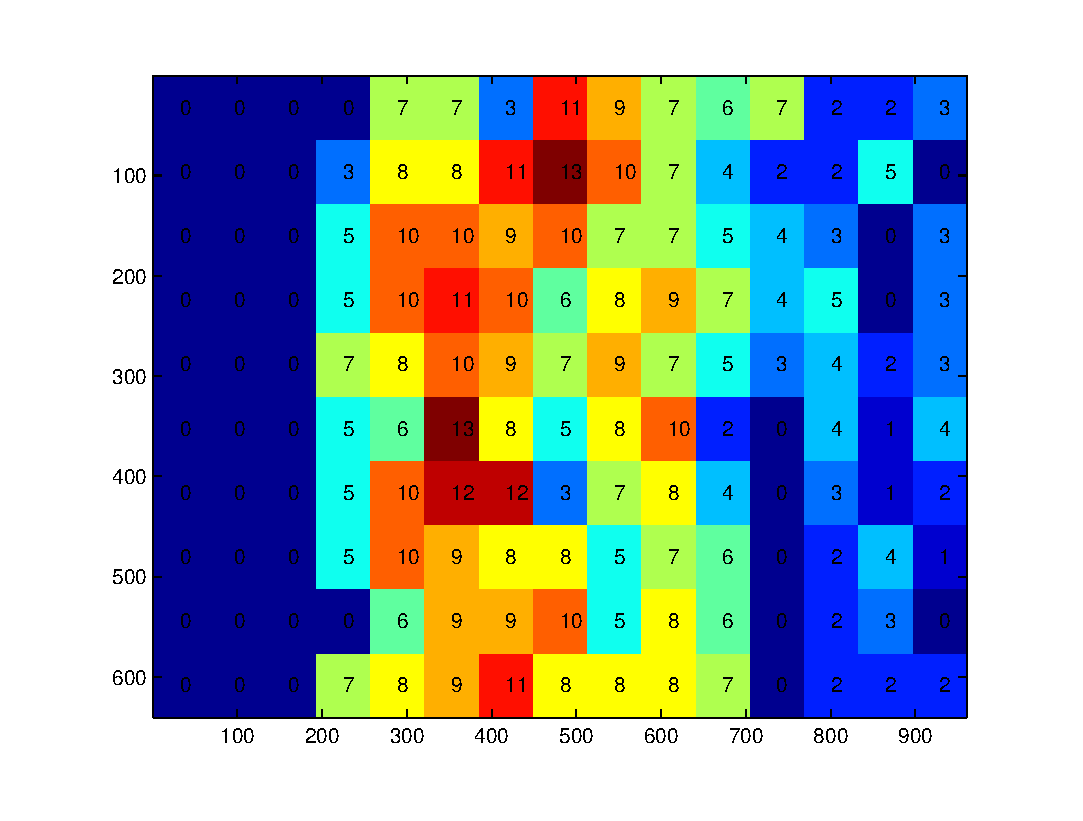
\includegraphics[width=\textwidth]{figures/mrf_true.eps}
          \caption{True Density}
        \end{subfigure}
        ~
        \begin{subfigure}[b]{0.3\textwidth}
	  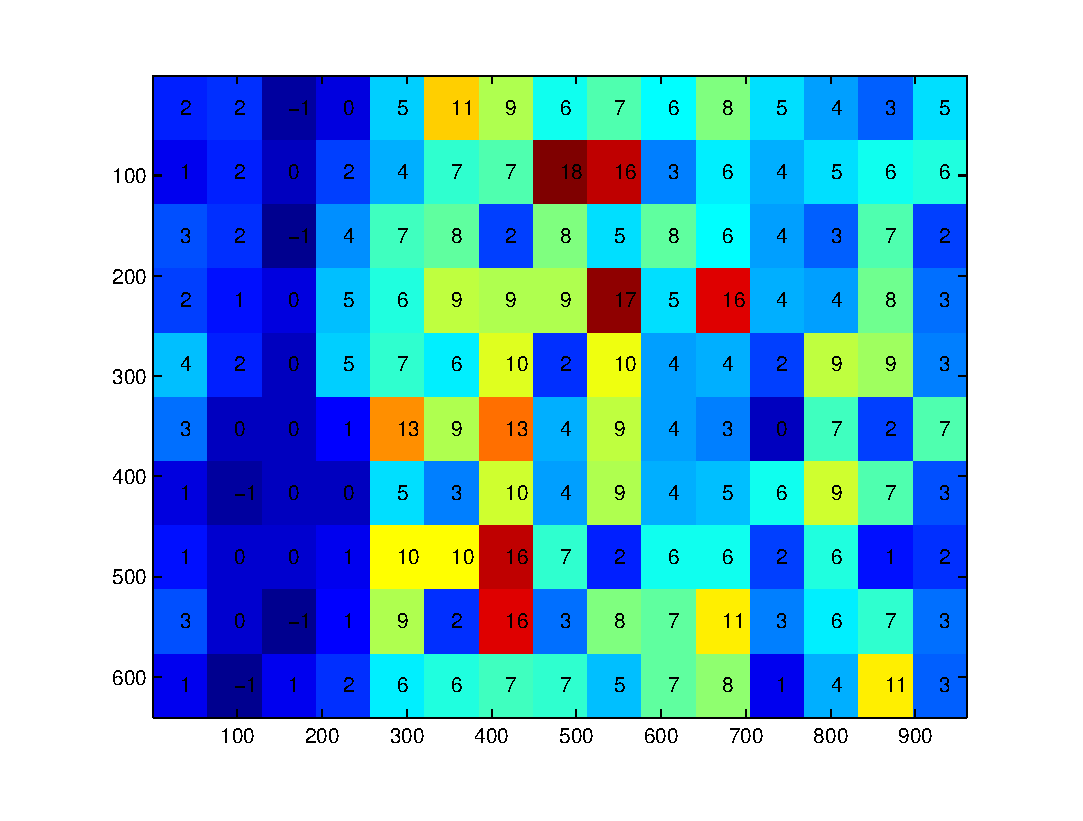
\includegraphics[width=\textwidth]{figures/mrf_before.eps}
          \caption{Estimated Density before MRF}
        \end{subfigure}
        ~
        \begin{subfigure}[b]{0.3\textwidth}
	  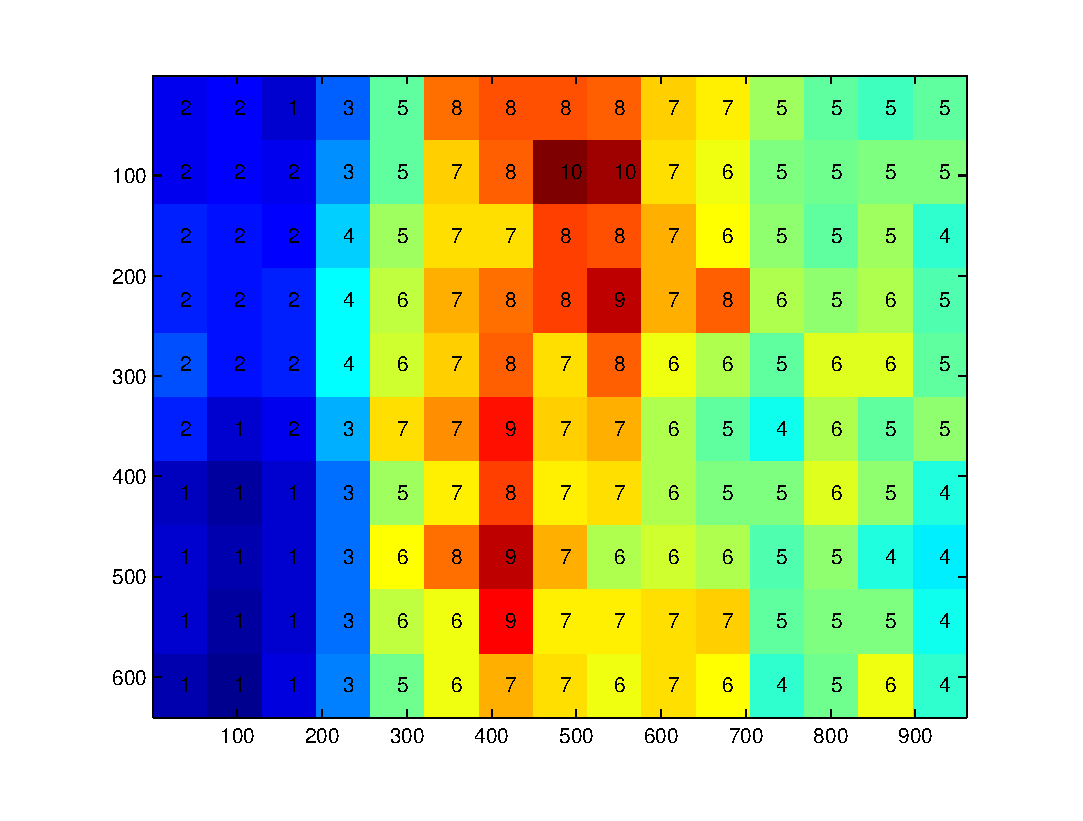
\includegraphics[width=\textwidth]{figures/mrf_after.eps}
          \caption{Estimated Density after MRF}
        \end{subfigure}
\end{figure}

\section*{Conclusion}
We managed to improve the results on cells counting from the method described in \cite{basepaper}, by replacing SIFT features with CNN features \cite{overfeat}. The results we obtained were without any specific retraining of the network, which means further improvements might be achieved this way. For crowd counting, replacing SIFT with CNN features also led to significant improvement over \cite{basepaper}, but less so compared to \cite{multisource}.

\bibliography{../proposal/biblio}
\end{document}